\section{Results}
\label{sec:results}

This section reports objective wrap-repair scores under locked $R_{\mathrm{blend}}$
(Sections~\ref{sec:v10-freeze}--\ref{sec:n2n-vs-ours-boards}).
Higher is better. Unless noted, multi-seed cells are mean$\pm$std.
Appendix~\ref{app:supplement} holds the matched outer-loop bake-off, ablations, HP probes, and transfer latency.
Limitations are collected in Section~\ref{sec:limitations}.
The evaluation protocol is stated in Section~\ref{sec:experiments}.

\paragraph{How to read the main numbers.}
\begin{enumerate}
  \item \textbf{Holdout vs Noise2Noise and Dual Cosine} (Table~\ref{tab:n2n-vs-ours}):
    short-FitCell hybrid is close to, but below, Noise2Noise, and far above Dual Cosine.
  \item \textbf{Which outer loop to keep} (Table~\ref{tab:meta-approaches}):
    hybrid wins a matched $5$k bake-off, so later compute goes to hybrid alone.
  \item \textbf{Longer FitCell} (Table~\ref{tab:v14-hybrid-converge}):
    one search seed logs in-loop $R_{\mathrm{blend}}$ above the frozen holdout Noise2Noise gate (provisional; multi-seed pending).
  \item \textbf{Where classical fails} (Section~\ref{sec:cliff-strata}):
    hard wrap cliffs collapse Dual Cosine; searched operators and Noise2Noise hold.
\end{enumerate}

\begin{figure}[t]
  \centering
  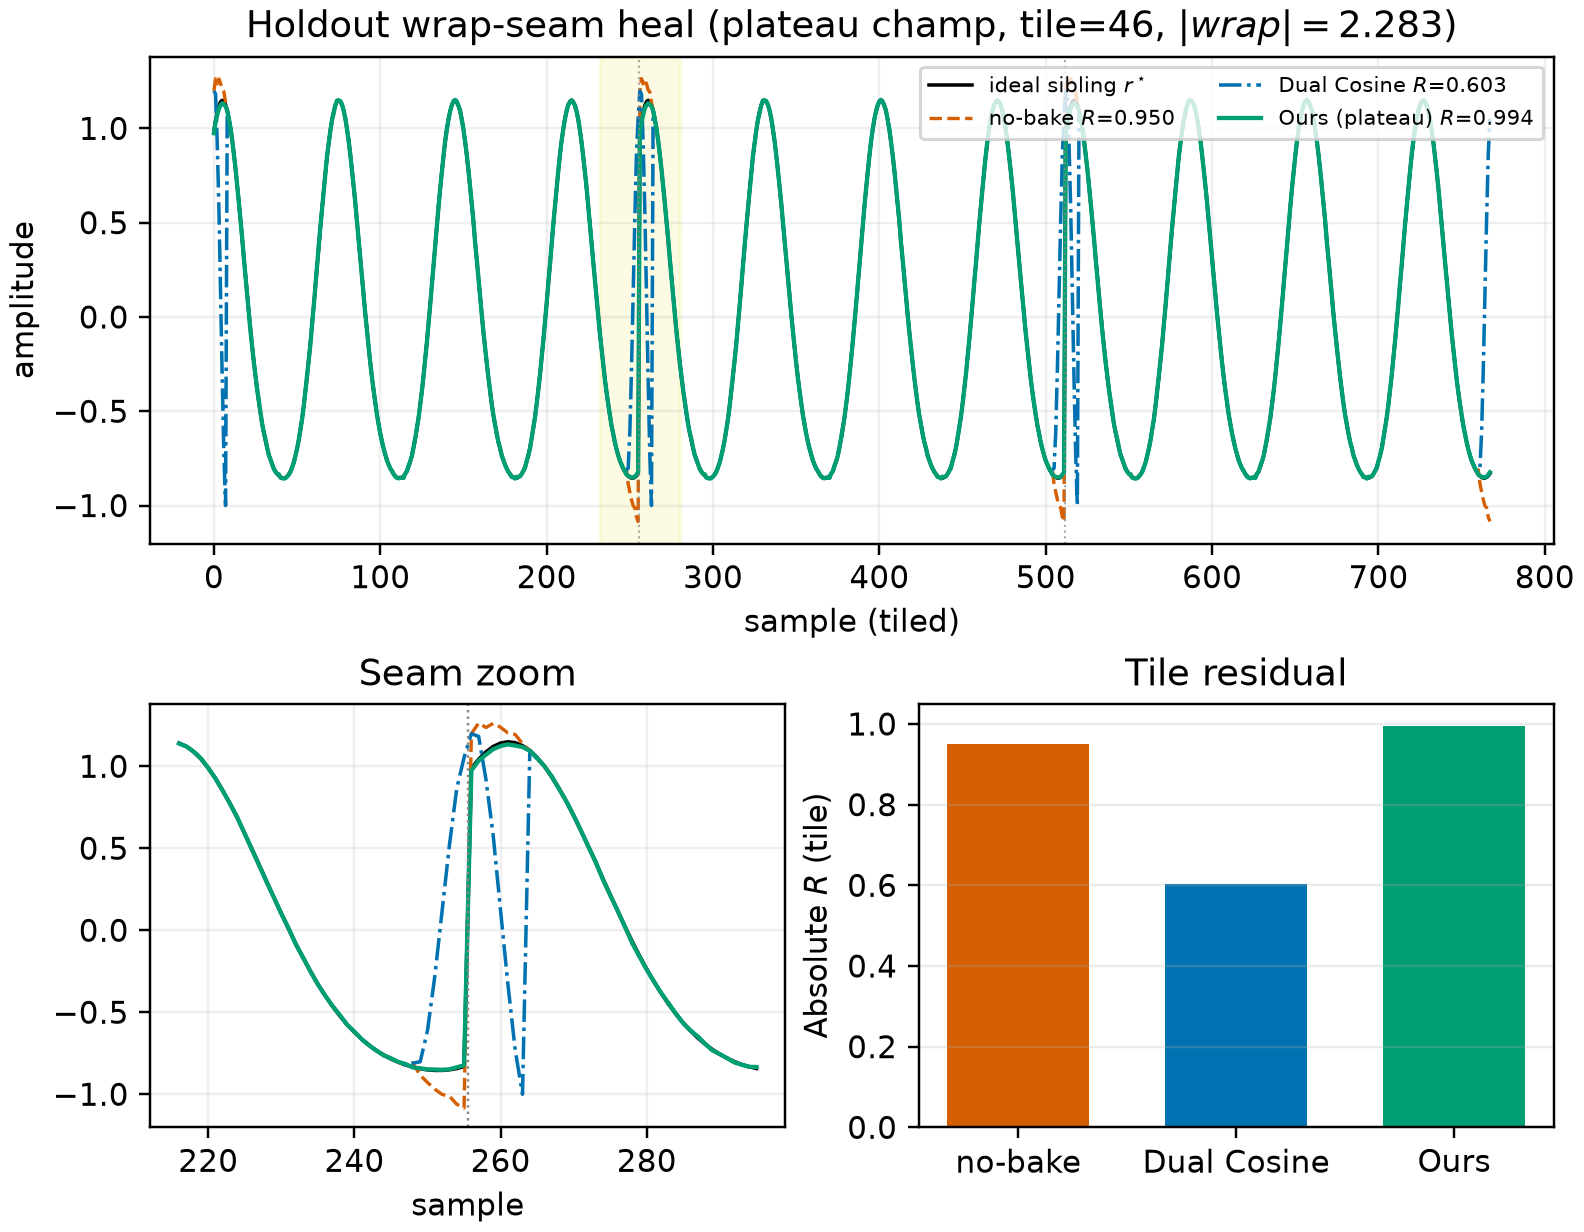
\includegraphics[width=\columnwidth]{figures/fig_meta_heal_samples.png}
  \caption{Holdout wrap-seam heal for the FitCell-to-plateau hybrid champion ($R_{\mathrm{blend}}{\approx}0.9912$, seed \texttt{1902771841}) vs no-bake, Dual Cosine, and ideal sibling $r^{\star}$.}
  \label{fig:meta-heal-samples}
\end{figure}

\subsection{A short hybrid search under $R_{\mathrm{blend}}$}
\label{sec:v10-freeze}

We first ask whether a hybrid GA+PPO search can beat frozen Noise2Noise under $R_{\mathrm{blend}}$ and $J$.
A $1{,}200$-iteration run (seed \texttt{1902771841}, ${\approx}1.65$\,h) selects on $J$~\eqref{eq:outer-obj} with $\lambda{=}0.02$.
The champion reaches $R_{\mathrm{blend}}{\approx}0.9695$ ($J{\approx}0.9603$, $t{\approx}5.08$\,ms).
Dual Cosine on the same runner scores ${\approx}0.504$.
The frozen Noise2Noise holdout gate is ${\approx}0.9750$.
So this short search clears Dual Cosine but not Noise2Noise.
Artifacts:
\href{https://github.com/reeldemo/denoise-opt-meta/blob/master/paper/Unsupervised_Wrap-Discontinuity_Repair_in_Wavetable_Synthesis_via_Hybrid_GA-PPO_Meta-Search_v12/figures/meta_approach_compare_v10.json}{hybrid search data}.

\subsection{Noise2Noise vs Ours on four boards}
\label{sec:n2n-vs-ours-boards}

Table~\ref{tab:n2n-vs-ours} is the main comparison under locked $R_{\mathrm{blend}}$.
Dual Cosine is the classical fade on every board.
Noise2Noise is the primary neural gate for this protocol (not a DenoiseOpt variant).

\paragraph{Holdout.}
Over five evaluation seeds (\texttt{20260719}--\texttt{20260723}), Noise2Noise leads the short-FitCell hybrid on every seed:
$0.9767{\pm}0.0015$ vs $0.9708{\pm}0.0014$.
Dual Cosine sits at $0.542{\pm}0.038$.
The hybrid is therefore competitive with Noise2Noise and far better than a classical fade, but it does not win the holdout gate under short FitCell.

\paragraph{Multi-family board.}
On twenty generative waveforms, board means are close:
Ours $0.9337{\pm}0.0028$, Noise2Noise $0.9308{\pm}0.0045$
(mean win fraction $0.47$; sign test on board-mean deltas $p{=}1.0$).
That is no significant mean difference. Both beat Dual Cosine.

\paragraph{Factory and AKWF.}
On wavetable-native corpora ($n{=}1{,}280$ each), Noise2Noise leads both Factory+FX
($0.771$ vs Ours $0.699$; Dual Cosine $0.589$)
and AKWF
($0.731$ vs Ours $0.679$; Dual Cosine $0.424$).

\begin{table}[htbp]
  \centering
  \caption{Parameter count and inference latency under the locked holdout story.
    Favorite $\Theta$ is the v10.1 hybrid champion (search seed \texttt{1902771841}).
    SeamN2N is the frozen corrupt$\to$corrupt gate (train seed \texttt{424242}).
    Holdout $R_{\mathrm{blend}}$ is mean$\pm$std over five evaluation seeds.
    Latency is CUDA ms/batch at $B{=}64$ (Table~\ref{tab:ours-n2n-latency}).}
  \label{tab:param-fairness}
  \setlength{\tabcolsep}{4pt}
  \begin{adjustbox}{max width=\columnwidth}
\begin{tabular}{@{}lrrr@{}}
    \toprule
    Method & Params & Holdout $R_{\mathrm{blend}}$ & ms/$B{=}64$ \\
    \midrule
    Favorite $\Theta$ (v10.1 hybrid) & ${\approx}121$k & $0.9708{\pm}0.0014$ & $8.20$ \\
    SeamN2N (corrupt$\to$corrupt) & ${\approx}53.5$k & $0.9767{\pm}0.0015$ & $1.12$ \\
    Dual Cosine & $0$ & $0.542{\pm}0.038$ & --- \\
    \bottomrule
  \end{tabular}
\end{adjustbox}
\end{table}

Table~\ref{tab:param-fairness} shows size and speed.
The hybrid favorite is larger and about $7.4\times$ slower per holdout batch than SeamN2N.
That is partly by design: selection maximizes $J=R_{\mathrm{blend}}-\lambda\cdot\mathrm{latency\_norm}$,
so a slower cell can win when residual gains outweigh the $\lambda$ penalty.
We do not claim architectural superiority over Noise2Noise on this freeze.
Search seeds, the N2N train seed \texttt{424242}, and holdout seeds remain disjoint.

\paragraph{Seed protocol.}
Holdout and multi-family rows in Table~\ref{tab:n2n-vs-ours} use five evaluation seeds.
The matched $5$k outer-loop bake-off uses three search seeds
(Table~\ref{tab:meta-approaches}: hybrid $0.9748{\pm}0.0018$, Aging $0.9635{\pm}0.0049$).

\subsection{Hybrid-only FitCell-to-convergence}
\label{sec:v14-converge}
\label{sec:v14-hybrid-converge}

The matched bake-off (Table~\ref{tab:meta-approaches}) already ranked hybrid first under a short FitCell budget (${\approx}16$--$48$ steps).
We therefore stop spending matched budget on Random, CMA-ES, TPE, Aging, and REINFORCE.
The follow-up is hybrid-only FitCell-to-plateau: every candidate trains until residual plateau
(or a searchable hard cap $T_{\max}\!\in\!\{512,\ldots,2048\}$),
with searchable patience, relative $\varepsilon$, batch size, and $\lambda$
(artifacts \texttt{meta\_approach\_compare\_v14\_converge/}).

The outer budget is $750$ evaluations with two sequential proposals per iteration on one GPU.
On \textbf{search seed} \texttt{1902771841} only, the champion logs in-loop $R_{\mathrm{blend}}{\approx}0.9912$
($J{\approx}0.9854$, $t{\approx}8.70$\,ms) after ${\approx}46.9$\,h wall on fresh procedural evaluation batches during the converge campaign.
That score is \emph{not} the five-seed holdout mean (Table~\ref{tab:n2n-vs-ours}); it is compared against the frozen holdout Noise2Noise gate (${\approx}0.9750$; train seed \texttt{424242}, eval seed \texttt{20260719}).
We treat ``clears the gate'' as \textbf{provisional} until FitCell-to-plateau runs complete for search seeds \texttt{2026072701} and \texttt{2026072702} and holdout replication is reported (Table~\ref{tab:compute-n2n-hybrid}, TBD rows).
Figure~\ref{fig:v14-converge-curve} shows the learning curve; Table~\ref{tab:v14-hybrid-converge} summarizes the freeze.

\begin{figure}[t]
  \centering
  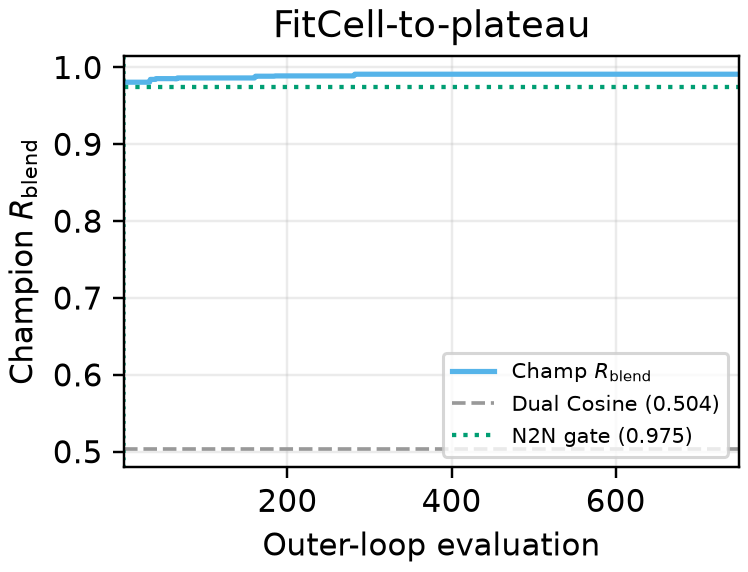
\includegraphics[width=0.92\columnwidth]{figures/fig_v14_converge_learning_curve.png}
  \caption{Hybrid FitCell-to-plateau learning curve (seed \texttt{1902771841}, $750$ evaluations).
  Champion $R_{\mathrm{blend}}$ vs.\ outer-loop evaluation with the frozen Noise2Noise gate
  (y-axis zoomed to the high-$R$ regime; Dual Cosine sits far below).
  Final champion $R_{\mathrm{blend}}{\approx}0.9912$.}
  \label{fig:v14-converge-curve}
\end{figure}

\begin{table}[t]
  \centering
  \caption{Hybrid FitCell-to-plateau under locked $R_{\mathrm{blend}}{+}J$
  (search seed \texttt{1902771841}, $750/750$ in-loop evaluations).
  Gate: frozen holdout Noise2Noise $R_{\mathrm{blend}}{\approx}0.9750$ (not an in-loop score).
  Provisional pending multi-search-seed replication.}
  \label{tab:v14-hybrid-converge}
  \setlength{\tabcolsep}{3pt}
  \footnotesize
  \begin{adjustbox}{max width=\columnwidth}
  \begin{tabular}{@{}lrrrc@{}}
    \toprule
    Setting & Iters & $R_{\mathrm{blend}}$ & $t$\,ms & vs N2N gate \\
    \midrule
    FitCell-to-plateau & $750/750$ & $0.9912$ & $8.70$ & clears \\
    Short FitCell (ref.) & $1{,}200$ & ${\approx}0.9695$ & ${\approx}5.08$ & below \\
    Frozen N2N gate & --- & ${\approx}0.9750$ & --- & --- \\
    \bottomrule
  \end{tabular}
  \end{adjustbox}
\end{table}

\subsection{Ablations and hyperparameter checks}
\label{sec:ablation-def}
\label{sec:ablation-hp-main}

Two narrow checks sit in Appendix~\ref{app:supplement}; they do not replace Table~\ref{tab:meta-approaches}.

\textbf{Ablations.}
We either (A)~read branch tags inside one recorded hybrid history, or
(B)~restart a short $150$-iteration search with GA-only, PPO-only, GA+PPO, or full hybrid
(Table~\ref{tab:ablation}; seed \texttt{1902771841}).
Type~B does not collapse short-budget $R_{\mathrm{blend}}$ when GA or PPO is dropped on that probe,
but those scores stay well below the matched-$5$k hybrid mean.

\textbf{Hyperparameters.}
A one-at-a-time $\pm 50\%$ probe at $500$ iterations moves champion $R$ by at most ${\approx}0.012$
(Table~\ref{tab:hp-sensitivity}).
Defaults are not claimed globally optimal.

\subsection{Ours vs Noise2Noise inference latency}
\label{sec:ours-n2n-latency}

Table~\ref{tab:ours-n2n-latency} compares CUDA forward time across boards and batch sizes.
At the default batch $B{=}64$, Ours is about $7\times$ slower than Noise2Noise on every board
(holdout $8.20$ vs $1.12$\,ms; multi-family mean $7.50{\pm}0.56$ vs $1.06{\pm}0.07$\,ms).
A holdout batch sweep ($B\in\{1,8,64,256\}$) keeps the ratio near $5$--$7\times$.
Larger batches help both methods, but Noise2Noise stays faster.
This matches the parameter gap (${\approx}121$k vs ${\approx}53.5$k) and the $J$ latency term in~\eqref{eq:outer-obj}.
Artifacts: \texttt{v13\_ours\_vs\_n2n\_latency/latency\_compare.json}.

\begin{table}[t]
  \centering
  \caption{Inference latency: Ours vs Noise2Noise on CUDA (warmup 8, timed 30).
    Ratio $=$ Ours/N2N ms/batch.}
  \label{tab:ours-n2n-latency}
  \setlength{\tabcolsep}{3pt}
  \scriptsize
  \begin{tabular}{@{}lrrr@{}}
    \toprule
    Board / batch & Ours & N2N & Ratio \\
    \midrule
    Holdout ($B64$) & 8.20 & 1.12 & $7.4\times$ \\
    Multi-family ($B64$) & $7.50{\pm}0.56$ & $1.06{\pm}0.07$ & $7.1\times$ \\
    Factory+FX ($B64$) & 7.31 & 1.06 & $6.9\times$ \\
    AKWF ($B64$) & 7.50 & 1.11 & $6.7\times$ \\
    Holdout ($B1$) & 8.52 & 1.30 & $6.6\times$ \\
    Holdout ($B8$) & 7.71 & 1.07 & $7.2\times$ \\
    Holdout ($B256$) & 7.62 & 1.52 & $5.0\times$ \\
    \bottomrule
  \end{tabular}
\end{table}

\subsection{Search efficiency (learning curves)}
\label{sec:search-learning-curve}

Figure~\ref{fig:search-learning-curve} plots champion score against outer-loop evaluations
on seed \texttt{1902771841}.
The top panel is the short FitCell hybrid under locked $R_{\mathrm{blend}}{+}J$ ($1{,}200$ evaluations):
raw $R_{\mathrm{blend}}$ clears Dual Cosine immediately and plateaus below the Noise2Noise gate (${\approx}0.975$).
The bottom panel is the FitCell-to-plateau follow-up ($750$ evaluations):
the same outer loop continues until residual plateau (final in-loop $R_{\mathrm{blend}}{\approx}0.9912$ on seed \texttt{1902771841}; Section~\ref{sec:v14-converge}; provisional vs holdout).
The matched multi-seed $R_{\mathrm{blend}}$ bake-off is in Table~\ref{tab:meta-approaches}.
Live hybrid champions stay compact (${\approx}24$k$\pm$2k params across short-FitCell seeds), while mid-search graphs can swing from ${\approx}15$k to ${\approx}370$k.

\begin{figure}[t]
  \centering
  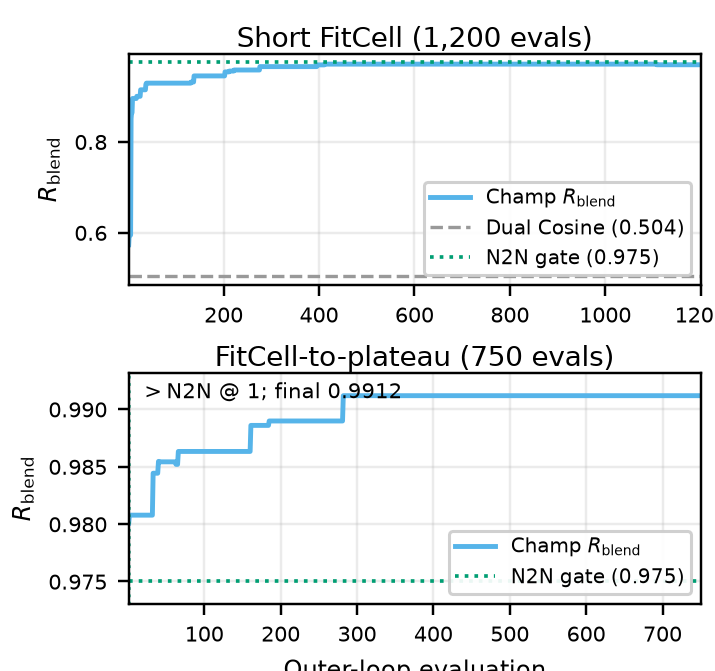
\includegraphics[width=0.92\columnwidth]{figures/fig_search_learning_curve.png}
  \caption{Hybrid search learning curves under $R_{\mathrm{blend}}$ (seed \texttt{1902771841}).
    Top: short FitCell ($1{,}200$ evaluations; champ.\ ${\approx}0.9695$; Dual Cosine + N2N gate).
    Bottom: FitCell-to-plateau ($750$ evaluations; champ.\ ${\approx}0.9912$; y-axis zoomed to the high-$R$ regime).}
  \label{fig:search-learning-curve}
\end{figure}

\begin{table}[t]
  \centering
  \caption{Ours vs Noise2Noise and Dual Cosine under $R_{\mathrm{blend}}$ ($\alpha{=}0.7$).
    Holdout / multi-family: mean$\pm$std over five seeds (\texttt{20260719}--\texttt{20260723}).
    $\Delta$ $=$ Ours $-$ baseline.}
  \label{tab:n2n-vs-ours}
  \setlength{\tabcolsep}{2.5pt}
  \scriptsize
  \begin{tabular}{@{}lrrrrr@{}}
    \toprule
    Board & Ours & N2N & DualCos. & $\Delta_{\mathrm{N2N}}$ & $\Delta_{\mathrm{DC}}$ \\
    \midrule
    Holdout & $0.971{\pm}0.001$ & $0.977{\pm}0.001$ & $0.542{\pm}0.038$ & $-0.006$ & $+0.429$ \\
    Multi-family & $0.934{\pm}0.003$ & $0.931{\pm}0.005$ & --- & $+0.003$ & --- \\
    Factory+FX & 0.699 & 0.771 & 0.589 & $-0.072$ & $+0.110$ \\
    AKWF OA & 0.679 & 0.731 & 0.424 & $-0.051$ & $+0.255$ \\
    \bottomrule
  \end{tabular}
\end{table}

\subsection{Hard cliffs expose classical fade failure}
\label{sec:cliff-strata}

On the top-10\% wrap-jump stratum of the holdout draw (seed \texttt{20260719}), Dual Cosine $R_{\mathrm{blend}}$ collapses ($0.525\to0.305$) while the short-FitCell hybrid and Noise2Noise hold ($0.971\to0.978$ and $0.976\to0.983$).
Seam-local edge RMSE on that stratum is in Table~\ref{tab:cliff-edge-rmse}; full stratification is Appendix Table~\ref{tab:cliff-strata}.

\begin{table}[t]
  \centering
  \caption{Edge RMSE on top-10\% wrap-jump tiles ($n{=}410$; lower better).}
  \label{tab:cliff-edge-rmse}
  \setlength{\tabcolsep}{6pt}
  \begin{tabular}{@{}lr@{}}
    \toprule
    Method & top10 edge RMSE \\
    \midrule
    N2N corrupt$\to$corrupt & 0.020 \\
    neural favorite & 0.027 \\
    no-bake & 0.095 \\
    DualCosine & 0.990 \\
    \bottomrule
  \end{tabular}
\end{table}

% Secondary tables (canonical classical board, VA seam, factory export, Rust bench) moved to Appendix~\ref{app:secondary-results}. Cross-domain transfer boards moved to Appendix~\ref{app:transfer-bundle}.
